\documentclass[11pt,a4paper]{article}
\usepackage[T1]{fontenc}
\usepackage[utf8]{inputenc}
\usepackage{lmodern,amsmath,amssymb,mathtools,mathrsfs,bm,booktabs,array,microtype,graphicx,xcolor,hyperref,siunitx}
\usepackage[a4paper,margin=24mm]{geometry}
\newcolumntype{P}[1]{>{\raggedright\arraybackslash}p{#1}}
\usepackage{pgfplots}
\pgfplotsset{compat=1.18}
\hypersetup{colorlinks=true,linkcolor=blue!45!black,citecolor=blue!45!black,urlcolor=blue!45!black,
  pdftitle={SST VAM-5 SST-17 Integrated Euler Director Action v0.2.0 DEVELOPMENT},pdfauthor={SST technical reconstruction}}
\newcommand{\rhoF}{\rho_{\!f}}
\newcommand{\rhoE}{\rho_{\!E}}
\newcommand{\rhoM}{\rho_{\!m}}
\newcommand{\rhoD}{\rho_{\!d}}
\newcommand{\rc}{r_c}
\newcommand{\vswirl}{\mathbf{v}_{\!\boldsymbol{\circlearrowleft}}}
\newcommand{\om}{\boldsymbol\omega}
\newcommand{\XX}{\mathbf X}
\newcommand{\qq}{\mathbf q}
\newcommand{\vv}{\mathbf v}
\newcommand{\dd}{\mathrm d}
\newcommand{\Dt}{\mathrm D_t}
\newcommand{\bb}{\mathbf b}
\newcommand{\EE}{\mathbf E}
\newcommand{\BB}{\mathbf B}
\newcommand{\status}{\textcolor{red!65!black}{DEVELOPMENT / NOT PHYSICALLY CERTIFIED}}
\begin{document}
\title{An Integrated Constrained Euler--Director Action for SST:\\
\large A Mathematically Traceable Repair of VAM-5 and SST-17}
\author{Technical reconstruction of manuscripts by O. Iskandarani\\\small SST-Workbench research artifact; original papers preserved unchanged}
\date{20 October 2026 --- v0.2.0 --- \status}
\begin{abstract}
We integrate the 2025 VAM-5 vortex-based Lagrangian programme and the 2026 SST-17 torsion-photon proposal without promoting their electrodynamic, relativistic or gravitational hypotheses to derived laws. A constrained Lagrangian-material action couples incompressible Euler flow to an additional transverse director-like displacement $\qq$ with independent inertia $\rhoD$ and stiffness $K$. We give the full action, variational equations, stress and canonical Hamiltonian, and show that its frozen-background transverse linear sector maps to \emph{source-free Maxwell equations} under an explicit dimensional field rescaling. A projected Cartan-torsion representation is a kinematic embedding of the same closed two-form, not a new derivation of Maxwell dynamics. An optional gyroscopic term realizes an optical-rotation toy model but requires an unverified physical mechanism relating background magnetic field to the gyroscopic frequency. Forty-seven automated unit, identity, local functional-derivative and linear-wave regression checks pass. No 3D coupled Euler--director evolution, PKLSA knot evolution, particle-mass closure, electromagnetic charge generation or observed photon phenomenology is certified here.
\end{abstract}
\maketitle
\tableofcontents
\clearpage

\section{Sources, research objective and boundaries}
The source documents are (i) VAM-5, \emph{On a Vortex-Based Lagrangian Unification of Gravity and Electromagnetism} (2025), particularly its Eqs.~(23)--(38) and helicity/charge arguments \cite{VAM5}; (ii) the independent constrained-Euler correction v0.1.0, issued as a DEVELOPMENT document on 20 October 2026 \cite{Repair01}; and (iii) SST-17, \emph{Electromagnetism as Propagating Torsion in a Hydrodynamic Vacuum} (17 January 2026), Eqs.~(1)--(16) \cite{SST17}. The original manuscripts are preserved as historical source material.

The physical premise used here is a Euclidean 3D inviscid fluid with absolute evolution time $t$, supplemented \emph{hypothetically} by director-like internal degrees of freedom. A strictly incompressible classical Euler fluid alone has no finite linear elastic shear modulus and does not produce the SST-17 photon wave equation. The new displacement variable and positive $K$ are therefore \emph{new model content}, not consequences of incompressibility or knotted vorticity. The present construction gives a consistent \emph{candidate action} in which their interactions with fluid deformation are specified and can be independently falsified.

\begin{table}[h]
\caption{Source-to-repair traceability. ``Algebraic mapping'' means an identity of chosen field equations, not an experimentally demonstrated derivation.}
\begin{tabular}{P{0.23\linewidth}P{0.34\linewidth}P{0.31\linewidth}}
Original claim & Mathematical issue or extra input & v0.2.0 disposition\\
\hline
VAM-5 unified $\mathcal L(\vv,\om)$ & Velocity-only local functional does not yield canonical momentum $\rhoF\vv$ with respect to $\dot\vv$ & Constrained material-map action and genuine momenta\\
VAM-5 pressure $\rightarrow$ gravity & Pressure acceleration is not automatically force on a separate object; no Newtonian closure & Euler pressure retained; gravity UNRESOLVED\\
VAM-5 helicity $\rightarrow$ charge & Coulomb kernel and conversion coefficient inserted, not derived & Charge/current sources excluded from vacuum sector\\
SST-17 $\rho_{\rm eff},K$ photon & Director elasticity and $c=\sqrt{K/\rho_{\rm eff}}$ require new constitutive dynamics & Explicit independent $\rhoD,K$ and calibrated wave limit\\
SST-17 $F=\kappa u_aT^a$ & Closedness follows from exterior derivative in restricted gauge, not propagation & Explicit kinematic embedding; wave dynamics comes from action\\
SST-17 Verdet $V\sim\alpha/2$ & Missing SI units and $\Omega(B)$ constitutive closure & Optional gyroscopic toy; $V=\beta/c$, $[\beta]=\mathrm{s^{-1}T^{-1}}$\\
\end{tabular}
\end{table}

\section{Notation, physical dimensions and explicit assumptions}
The fixed reference volume is $\Omega_0$ with material labels $a_A$; $\XX(\mathbf a,t)$ is the flow map; $F_{iA}=\partial_A X_i$, $J=\det F$, $G_{Ai}=(F^{-1})_{Ai}$. Physical positions are $\mathbf x=\XX(\mathbf a,t)$, fluid velocity is $\vv(\XX,t)=\dot\XX$, and $\om=\nabla_{\!x}\times\vv$.

An independent internal displacement $\qq(\mathbf a,t)\in\mathbb R^3$ has dimension $[\qq]=\mathrm m$; its gradient in physical coordinates is
\begin{equation}
D_iq_j:=\partial_{a_A}q_j\,G_{Ai},\qquad
b_k:=(\nabla_{\!x}\times\qq)_k=\varepsilon_{kij}D_iq_j,\qquad
h:=\nabla_{\!x}\cdot\qq=D_iq_i.
\label{eq:operators}
\end{equation}
The independent effective inertia density $\rhoD>0$ has units $\mathrm{kg\,m^{-3}}$; $K>0$ has units $\mathrm{Pa}=\mathrm{J\,m^{-3}}$. They are not interchangeable with $\rhoE$ (energy density), $\rhoM=\rhoE/c^2$ (mass-equivalent density) or $\rho_{\mathrm{core}}$ (historically postulated core density). The director $\qq$ is a \emph{small, vector-valued material displacement}, not yet a derived unit-length director, photon soliton, Maxwell four-potential or Cartan coframe.

We assume smooth invertible $\XX$, $J=1$, periodic boundary conditions or boundary conditions cancelling integrations by parts, uniform $\rhoF$, and smooth solutions. Pressure $p$ and $\eta$ below are Lagrange multipliers. These assumptions exclude reconnections, singular cores and unresolved physical boundaries; finite-core PKLSA implementation needs new qualification.

\section{Integrated material action and exact field variation}
\subsection{Action with incompressibility and transverse displacement constraint}
The proposed \emph{minimal integrated candidate} is
\begin{equation}
\boxed{\begin{aligned}
\mathcal A[\XX,\qq,p,\eta]=\int\!\dd t\int_{\Omega_0}\!\dd^3a\,\Big[
&\frac{\rhoF}{2}|\dot\XX|^2+\frac{\rhoD}{2}|\dot\qq|^2
-\frac K2|\bb|^2\\[-2pt]
&+p(J-1)+\eta h\Big],\qquad
J=\det F,\quad \bb=\nabla_{\!x}\times\qq,\quad h=\nabla_{\!x}\cdot\qq.
\end{aligned}}
\label{eq:action}
\end{equation}
The dependence of $\bb$ and $h$ on $\XX$ through $F^{-1}$ is a genuine \emph{mechanical coupling}: deforming the incompressible flow map changes the director elastic energy. A direct sum of separate fluid and wave actions would not have this response. Writing these terms per reference volume rather than multiplying by $J$ is an off-constraint convention; $J=1$ on shell, but off-constraint changes can shift the multiplier pressure. All reported stresses use the precise convention in Eq.~\eqref{eq:action}.

Variations of the multipliers give
\begin{equation}
\boxed{J=1,\qquad h=0.}
\label{eq:constraints}
\end{equation}
The first constraint is incompressibility; the second is a transverse field \emph{constraint} and should not be conflated with a demonstrated electromagnetic gauge symmetry.

\subsection{Director variation}
At fixed $\XX$, variation of $\qq$ uses $\delta\bb=\nabla\times\delta\qq$, $\delta h=\nabla\cdot\delta\qq$, and the Piola identity $\partial_A(JG_{Ai})=0$. On $J=1$ the Euler--Lagrange equation is
\begin{equation}
\boxed{\rhoD\,\ddot\qq+K\nabla_{\!x}\times\bb+\nabla_{\!x}\eta=0,\qquad
\nabla_{\!x}\cdot\qq=0.}
\label{eq:director}
\end{equation}
The double dot is the material time derivative at fixed label $\mathbf a$; thus $\ddot\qq$ is \emph{not} simply $\partial_t^2\qq(\mathbf x,t)$ in a moving flow. Spatial derivatives are evaluated using the instantaneous deformed map.

\subsection{Fluid-map variation and backreaction}
Let $Q_{jA}=\partial_Aq_j$. The identities $\delta J=JG_{Al}\delta F_{lA}$ and $\delta G_{Ai}=-G_{Al}\delta F_{lB}G_{Bi}$ give the Piola-like derivative
\begin{equation}
\boxed{\begin{aligned}
P_{lA}:=\frac{\partial\mathcal L}{\partial F_{lA}}=
&pJG_{Al}
+K b_k\varepsilon_{kij}(D_lq_j)G_{Ai}
-\eta(D_lq_i)G_{Ai}.
\end{aligned}}
\label{eq:piola}
\end{equation}
The integrated fluid map satisfies
\begin{equation}
\boxed{\rhoF\ddot X_l=-\partial_{a_A}P_{lA}.}
\label{eq:fluid}
\end{equation}
Equivalently, for $J=1$ its spatial form is
\begin{equation}
\rhoF\left[\partial_t v_l+(\vv\cdot\nabla)v_l\right]
=-\partial_lp-\partial_i\Big[K b_k\varepsilon_{kij}\partial_lq_j-\eta\partial_lq_i\Big].
\label{eq:fluid_spatial}
\end{equation}
No physical \emph{gravitational or electromagnetic force} has been presumed. The last divergence is the response of the candidate internal displacement elasticity and its constraint. In the consistent sector $\qq=0$, $\eta=0$, it vanishes and Eqs.~\eqref{eq:fluid}--\eqref{eq:constraints} reduce exactly to the familiar incompressible Euler system:
\begin{equation}
\boxed{\rhoF(\partial_t\vv+(\vv\cdot\nabla)\vv)=-\nabla p,\qquad \nabla\cdot\vv=0.}
\label{eq:euler}
\end{equation}
This is a direct model limit. The director backreaction is \emph{not} a consequence of bare Euler theory.

\subsection{Canonical Hamiltonian and conserved energy}
The canonical momenta are truly conjugate to material coordinates and to the new displacement:
\begin{equation}
\boxed{\mathbf P_X=\rhoF\dot\XX,\qquad \mathbf P_q=\rhoD\dot\qq.}
\end{equation}
The constrained Hamiltonian functional is
\begin{equation}
\mathscr H=\int_{\Omega_0}\!\dd^3a
\left[\frac{|\mathbf P_X|^2}{2\rhoF}
+\frac{|\mathbf P_q|^2}{2\rhoD}
+\frac K2|\bb|^2-p(J-1)-\eta h\right].
\label{eq:hamilton}
\end{equation}
On the constraint surface, the time-independent, boundary-flux-free system has non-negative conserved total energy
\begin{equation}
\boxed{E=\int_{\Omega_0}\!\dd^3a\left(\frac{\rhoF}{2}|\dot\XX|^2+\frac{\rhoD}{2}|\dot\qq|^2+\frac K2|\bb|^2\right).}
\label{eq:energy}
\end{equation}
The full canonical system remains constrained; this expression alone does not specify a numerically well-posed scheme or a finite-domain boundary prescription. Pressure and $\eta$ can be shifted by appropriate freedoms associated with their constraints. The numerical test suite checks the local derivatives in Eqs.~\eqref{eq:piola} and \eqref{eq:director} by independent central finite differences, rather than merely substituting the same formula on both sides.

\section{Free transverse sector and exact Maxwell-form correspondence}
Take the \emph{frozen reference background} $\XX(\mathbf a,t)=\mathbf a$, ignore fluid backreaction as a linear test-field approximation, and choose periodic boundary conditions. Then Eq.~\eqref{eq:director} becomes
\begin{align}
\rhoD\partial_t^2\qq+K\nabla\times(\nabla\times\qq)+\nabla\eta&=0,
&\nabla\cdot\qq&=0.\label{eq:wavepre}
\end{align}
Taking the divergence gives $\nabla^2\eta=0$; for periodic, zero-mean $\eta$ it vanishes. Thus
\begin{equation}
\boxed{\partial_t^2\qq-c_d^2\nabla^2\qq=0,
\quad \nabla\cdot\qq=0,\quad c_d^2=K/\rhoD.}
\label{eq:wavelin}
\end{equation}
This has two transverse polarizations; longitudinal excitations have been removed by the explicit constraint. The speed $c_d$ is an \emph{input ratio} and is not predicted by Euler.

For comparison with free electrodynamics let $\epsilon_0,\mu_0$ be the SI vacuum parameters and define a \emph{dimensional field calibration} $\zeta>0$ with units tesla. Define
\begin{equation}
\boxed{\EE=-\zeta\partial_t\qq,\qquad \BB=\zeta\nabla\times\qq,\qquad
\epsilon_0\zeta^2=\rhoD,\quad \frac{\zeta^2}{\mu_0}=K.}
\label{eq:EMmapping}
\end{equation}
The two calibration equalities require $K/\rhoD=1/(\epsilon_0\mu_0)=c^2$ and establish a source-free \emph{isomorphism}, not an explanation for the empirical constants. Consequently
\begin{equation}
\boxed{\begin{aligned}
\nabla\cdot\BB&=0, & \partial_t\BB+\nabla\times\EE&=0,\\
\nabla\cdot\EE&=0, & \partial_t\EE-c^2\nabla\times\BB&=0.
\end{aligned}}
\label{eq:maxwell}
\end{equation}
Furthermore the free director energy density maps exactly to the vacuum electromagnetic energy density:
\begin{equation}
\frac{\rhoD}{2}|\dot\qq|^2+\frac K2|\nabla\times\qq|^2
=\frac{\epsilon_0}{2}|\EE|^2+\frac1{2\mu_0}|\BB|^2.
\end{equation}
No electric charge, magnetic monopole, source current, gauge-invariant charged matter coupling, emergent photon quantization, or radiation from a finite-core PKLSA knot follows from this correspondence. In a \emph{moving or deformed} background the equations are not generically the usual flat-spacetime Maxwell system: material derivatives and fluid stresses remain and must be solved.

\section{Cartan torsion projection: exact identity versus independent physics}
In a local teleparallel gauge with a fixed coframe $\theta^a$, vanishing connection $\omega^a{}_b=0$, and projected \emph{constant} internal covector $u_a$, SST-17 writes
\begin{equation}
T^a=\dd\theta^a,\qquad \mathcal F=\kappa u_aT^a
=\dd(\kappa u_a\theta^a),\qquad \dd\mathcal F=0.
\label{eq:cartan}
\end{equation}
The last equation is $\dd^2=0$ and is \emph{kinematic}; the inhomogeneous Maxwell equations require an action. In the free temporal-gauge sector one may \emph{construct} a coframe perturbation so that the projected one-form is $\mathcal A=\zeta q_i\dd x^i$, whence $\mathcal F=\dd\mathcal A$ and its spatial and time components correspond to Eq.~\eqref{eq:EMmapping}. Such construction is not unique and does not derive an electromagnetic gauge potential from a source-native vortex.

When $u_a$ varies, $\dd(u_aT^a)=\dd u_a\wedge T^a$ even for $\dd T^a=0$ in this gauge, and closure is no longer automatic. Likewise arbitrary Cartan connections require the fully covariant Bianchi identities, not a naive statement $\dd T^a=0$. No claim of demonstrated physical teleparallel gravity is implied.

\section{Optional gyroscopic/birefringent candidate: a clearly separate extension}
SST-17 proposes a rotating-background splitting and a putative vacuum Verdet constant. A mathematically consistent \emph{toy} mechanism for a uniform imposed axial frequency $\boldsymbol\Omega$ is the additional material Lagrangian
\begin{equation}
\boxed{\Delta\mathcal L_{\rm gyro}=\rhoD(\boldsymbol\Omega\times\qq)\cdot\dot\qq,
\quad [\boldsymbol\Omega]=\mathrm{s^{-1}}.}
\label{eq:gyro}
\end{equation}
On the frozen background the modified equation reads
\begin{equation}
\rhoD\left(\partial_t^2\qq+2\boldsymbol\Omega\times\partial_t\qq\right)
+K\nabla\times\nabla\times\qq+\nabla\eta=0.
\label{eq:gyrowave}
\end{equation}
The gyroscopic force performs no work since $\dot\qq\cdot(\boldsymbol\Omega\times\dot\qq)=0$, so the quadratic energy in Eq.~\eqref{eq:energy} remains conserved for a fixed $\boldsymbol\Omega$ and suitable boundaries. For $\mathbf k\parallel\boldsymbol\Omega$ and circular transverse polarization,
\begin{equation}
\omega_\pm^2\mp2\Omega\omega_\pm=c_d^2k^2,
\qquad n_\pm=\frac{c_dk_\pm}{\omega}\simeq1\mp\frac{\Omega}{\omega}
\quad (|\Omega|\ll\omega),
\end{equation}
up to the choice of labels for the two helicities. This gives $|\Delta\theta|\simeq|\Omega|L/c_d$ for a uniform propagation distance $L$.

To promote it to a \emph{magnetic vacuum prediction} one must derive, rather than prescribe, a relation $\Omega=\beta B_\parallel$. If such a relation holds, the corresponding SI Verdet constant is
\begin{equation}
\boxed{V_{\rm vac}:=\frac{\Delta\theta}{B_\parallel L}=\frac{\beta}{c_d},
\qquad [V_{\rm vac}]=\mathrm{T^{-1}m^{-1}},\quad
[\beta]=\mathrm{s^{-1}T^{-1}}.}
\label{eq:verdet}
\end{equation}
A dimensionless prediction of $V\simeq\alpha_{\rm vac}/2$ cannot stand without a conversion scale. The gyroscopic term in Eq.~\eqref{eq:gyro} is \emph{not part of the minimal integrated action} and is neither obtained from unforced incompressible Euler dynamics nor a verified vacuum property. Comparing with parity-even quadratic-in-$B$ birefringence requires attention to medium/plasma contamination, instrumental rotation and the possibility of other parity-odd physics \cite{CFJ,EH,Unruh}.

\section{Canonical SST values and internal numerical checks}
The archived SST constants used for validation are
\begin{align}
|\vswirl|&=1.09384563\times10^6\ \mathrm{m\,s^{-1}},&
\rc&=1.40897017\times10^{-15}\ \mathrm{m},\\
\rhoF&=7.0\times10^{-7}\ \mathrm{kg\,m^{-3}},&
\rho_{\rm core}&=3.8934358266918687\times10^{18}\ \mathrm{kg\,m^{-3}}.
\end{align}
Choosing \emph{for a test only} $\rhoD=\rhoF$ and inserting observed vacuum $c=299792458\ \mathrm{m\,s^{-1}}$ requires
\begin{equation}
\boxed{K=\rhoD c^2=6.29128625116\times10^{10}\ \mathrm{Pa}.}
\label{eq:numerical}
\end{equation}
The large effective stiffness is a \emph{calibrated constitutive coefficient}; ordinary incompressible inviscid Euler theory supplies no such shear elasticity. The core density $\rho_{\rm core}$ is \emph{not} substituted for $\rhoD$ or $\rhoF$. The characteristic kinematic core frequency $|\vswirl|/\rc$ is not identified with an independently measured photon or Swirl-Clock mode.

\section{Executable validation and precise evidence scope}
The accompanying cross-platform test harness evaluates 47 regressions and writes machine-readable results. These include SI dimensions; rigid-rotation Euler/pressure-Poisson controls; exact Galilean covariance of the uncoupled Euler limit; finite-difference differentiation of the \emph{local coupled action} with respect to both deformation $F$ and the director label gradient $Q$; objectivity under rigid rotations; two transverse free-wave polarizations; Maxwell closure and energy rescaling; gyroscopic branch relations; and a spectral 1D transverse wave mode evolved at three time resolutions.

\begin{figure}[h]
\centering
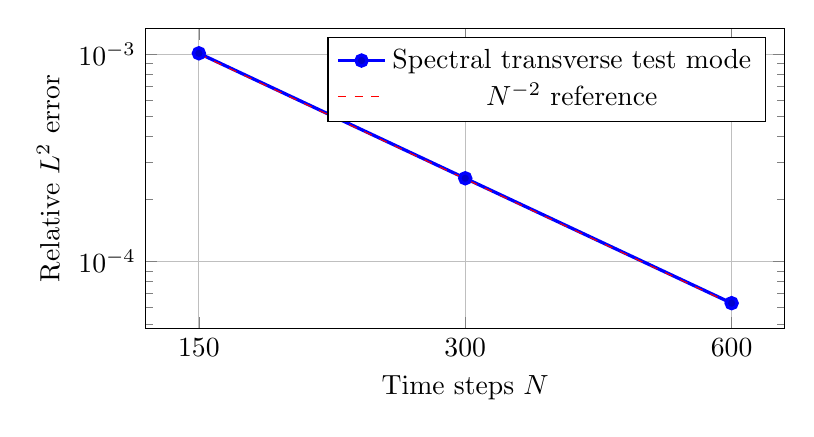
\begin{tikzpicture}
\begin{axis}[width=0.80\linewidth,height=5.4cm,xmode=log,ymode=log,xlabel={Time steps $N$},ylabel={Relative $L^2$ error},grid=major,xtick={150,300,600},xticklabels={150,300,600},legend pos=north east]
\addplot+[mark=*,very thick] coordinates {(150,0.0010093902) (300,0.0002519830) (600,0.0000629730)};
\addlegendentry{Spectral transverse test mode}
\addplot+[mark=none,dashed] coordinates {(150,0.0010) (600,0.0000625)};
\addlegendentry{$N^{-2}$ reference}
\end{axis}
\end{tikzpicture}
\caption{Second-order temporal convergence on a \emph{frozen-fluid, 1D transverse plane-wave} test. This is not coupled 3D Euler--director dynamics or a PKLSA finite-core knot.}
\end{figure}

\begin{table}[h]
\caption{Qualification gates; the tests report their own run status. ``PASS'' is never a claim of physical validation.}
\begin{tabular}{P{0.15\linewidth}P{0.55\linewidth}P{0.22\linewidth}}
Gate & Evidence requirement & Current status\\ \hline
G0 & Source traceability; dimensional and algebraic checks & PASS (analytic)\\
G1 & Variation and local Piola/director-gradient finite differences & PASS (local derivatives)\\
G2 & Free transverse Maxwell-form identities; time convergence & PASS (linear test)\\
G3 & Gyroscopic $\Omega(B)$ generated from native fluid/director physics & NOT RUN / UNKNOWN\\
G4 & Fully coupled 3D $\XX,\qq$ solver; energy, divergence and grid/time convergence & NOT RUN\\
G5 & Real PKLSA finite-core seed, knot provenance, topology and solver parity & NOT RUN\\
G6 & Charge, gravity, particle spectrum, quantum spin and Swirl Clock & UNRESOLVED\\
\end{tabular}
\end{table}

\section{PKLSA handoff contract and explicit falsifiers}
This DEVELOPMENT package is intentionally \emph{not} a fictitious PKLSA runner. A production connector should load only real source-native knot geometries, source checksums, circulation/core descriptors, physical background conditions and converged finite-core Biot--Savart/Euler fields; then extend the solver to the \emph{new independent} $\qq$ field and its backreaction stress. Suggested baseline families are $0_1$, $3_1$ and its true mirror, plus held-out Fourier, historical and relaxed PKLSA sources. Disjoint family/geometry splits must remain explicit.

The first physical falsifiers should be: (F1) a full-field Galilean boost leaves material intrinsic clocks unchanged, (F2) the $\qq\to0$ limit reproduces existing validated Euler source fields, (F3) a wave propagates only if an independently measured $\rhoD,K$ closure exists, (F4) the nonzero director backreaction satisfies both mechanical energy exchange and total conservation, (F5) emission/absorption requires a consistent source current rather than a constructed Coulomb kernel, and (F6) any $\Omega\propto B$ rotation is distinguishable from lab-frame Coriolis and ordinary medium effects. All parameter fitting must occur \emph{outside} blind evaluation families. The canonical SST symbols and force limits are unaffected by the present test.

\section{Conclusion and non-promotion rule}
Within this technical model, the old VAM-5 Lagrangian is replaced by a mathematically variation-consistent Euler substrate with a separately declared elastic displacement field. The original SST-17 Maxwell wave equation is recovered, in a frozen uniform background, as a two-polarization \emph{source-free} effective-sector correspondence. The torsion projection explains the homogeneous equations kinematically; it does not add independent wave dynamics. A Verdet-like gyroscopic rotation can be made dimensionally consistent, but its physical $B\to\Omega$ coupling has not been derived. The package is therefore a successful \emph{formal repair and linear numerical diagnostic}, not a proof of photon, gauge, gravitational, quantum or mass unification. No direct edit of the original PDFs, SST Canon, Google Drive or frozen falsifier framework is made.

\paragraph*{Physical analogy for a younger reader.}
Water can carry an elastic toy string that wiggles as water moves. We can calculate the water and the wiggle with one bookkeeping rule; however, simply making the string wiggle at the speed of light does not show that water creates real light. The wiggle speed and its interaction with matter still have to be measured independently.

\begin{thebibliography}{99}
\bibitem{VAM5} O. Iskandarani (2025), ``On a Vortex-Based Lagrangian Unification of Gravity and Electromagnetism: From Knotted Aether Vorticity to Standard Model Reconstruction using Swirlclock Dynamics, Topological Charge, and Emergent Mass,'' preprint, \url{https://doi.org/10.5281/zenodo.15772858}.
\bibitem{SST17} O. Iskandarani (2026), ``Electromagnetism as Propagating Torsion in a Hydrodynamic Vacuum: A Geometric Unification via Cartan Structure Equations,'' SST-17 preprint, \url{https://doi.org/10.5281/zenodo.17677074}.
\bibitem{Repair01} SST Technical Reconstruction (2026), \emph{Constrained Vortex-Fluid Action: A Technical Repair of VAM-5}, v0.1.0 DEVELOPMENT, companion research package (20 October 2026), with original VAM-5 provenance retained.
\bibitem{Salmon1988} R. Salmon (1988), ``Hamiltonian Fluid Mechanics,'' \emph{Annual Review of Fluid Mechanics} \textbf{20}, 225--256, \url{https://doi.org/10.1146/annurev.fl.20.010188.001301}.
\bibitem{Holm1998} D. D. Holm, J. E. Marsden and T. S. Ratiu (1998), ``The Euler--Poincar\'e Equations and Semidirect Products with Applications to Continuum Theories,'' \emph{Advances in Mathematics} \textbf{137}, 1--81, \url{https://doi.org/10.1006/aima.1998.1721}.
\bibitem{Moffatt1969} H. K. Moffatt (1969), ``The Degree of Knottedness of Tangled Vortex Lines,'' \emph{Journal of Fluid Mechanics} \textbf{35}, 117--129, \url{https://doi.org/10.1017/S0022112069000991}.
\bibitem{Unruh} W. G. Unruh (1981), ``Experimental Black-Hole Evaporation?,'' \emph{Physical Review Letters} \textbf{46}, 1351--1353, \url{https://doi.org/10.1103/PhysRevLett.46.1351}.
\bibitem{CFJ} S. M. Carroll, G. B. Field and R. Jackiw (1990), ``Limits on a Lorentz- and Parity-Violating Modification of Electrodynamics,'' \emph{Physical Review D} \textbf{41}, 1231--1240, \url{https://doi.org/10.1103/PhysRevD.41.1231}.
\bibitem{EH} W. Heisenberg and H. Euler (1936), ``Folgerungen aus der Diracschen Theorie des Positrons,'' \emph{Zeitschrift f\"ur Physik} \textbf{98}, 714--732, \url{https://doi.org/10.1007/BF01343663}.
\end{thebibliography}
\end{document}
